\chapter{Mô phỏng Hệ thống Nios V và DMA}
\label{Chapter4}

Mô phỏng (Simulation) là một bước quan trọng trong quy trình thiết kế \acrshort{fpga}, cho phép xác minh chức năng của thiết kế phần cứng và sự tương tác giữa các thành phần trước khi triển khai lên phần cứng vật lý. Việc này giúp phát hiện lỗi sớm, tiết kiệm thời gian và công sức gỡ lỗi trên bo mạch. Chương này trình bày quy trình và các công cụ được sử dụng để mô phỏng hệ thống \acrshort{soc} Nios V/m tích hợp bộ điều khiển DMA tùy chỉnh.

\section{Công cụ Mô phỏng và Yêu cầu Môi trường}

Công cụ chính được sử dụng để mô phỏng hệ thống trong dự án này là \textbf{Questa Advanced Simulator} (trước đây là ModelSim-Intel FPGA Edition), một trình mô phỏng mạnh mẽ được cung cấp bởi Siemens.

Khác với \acrshort{nios2}, hệ thống \acrshort{niosv} không hỗ trợ Generate Testbench System với các phiên bản Quartus Prime Lite và Standard trên hệ điều hành Windows (và Intel cũng đã thông báo sẽ không hỗ trợ cho việc này trên hệ điều hành Windows \cite{intel-forum-simulation}). Có 2 cách để tạo testbench cho hệ thống \acrshort{niosv}:

\begin{enumerate}
    \item \textbf{Sử dụng Quartus Prime Pro:} Phiên bản Pro này có nhiều tính năng hơn, tuy nhiên phiên bản này tốn dung lượng ổ cứng từ 40-145 GB.
    \item \textbf{Generate Testbench System trên Linux:} Thực hiện cài đặt Quartus Prime Lite/Standard trên hệ điều hành Linux. Sau đó sử dụng Platform Designer để Generate Testbench System cho hệ thống \texttt{system.qsys}. Sau khi testbench được tạo trên Linux thành công (hình \ref{fig:04_01_UbuntuGenerateTestbenchSystem}), các tệp này có thể được sao chép sang môi trường Windows để thực hiện mô phỏng bằng QuestaSim/ModelSim trên Windows nếu muốn.
\end{enumerate}

\begin{figure}[htbp]
    \centering
    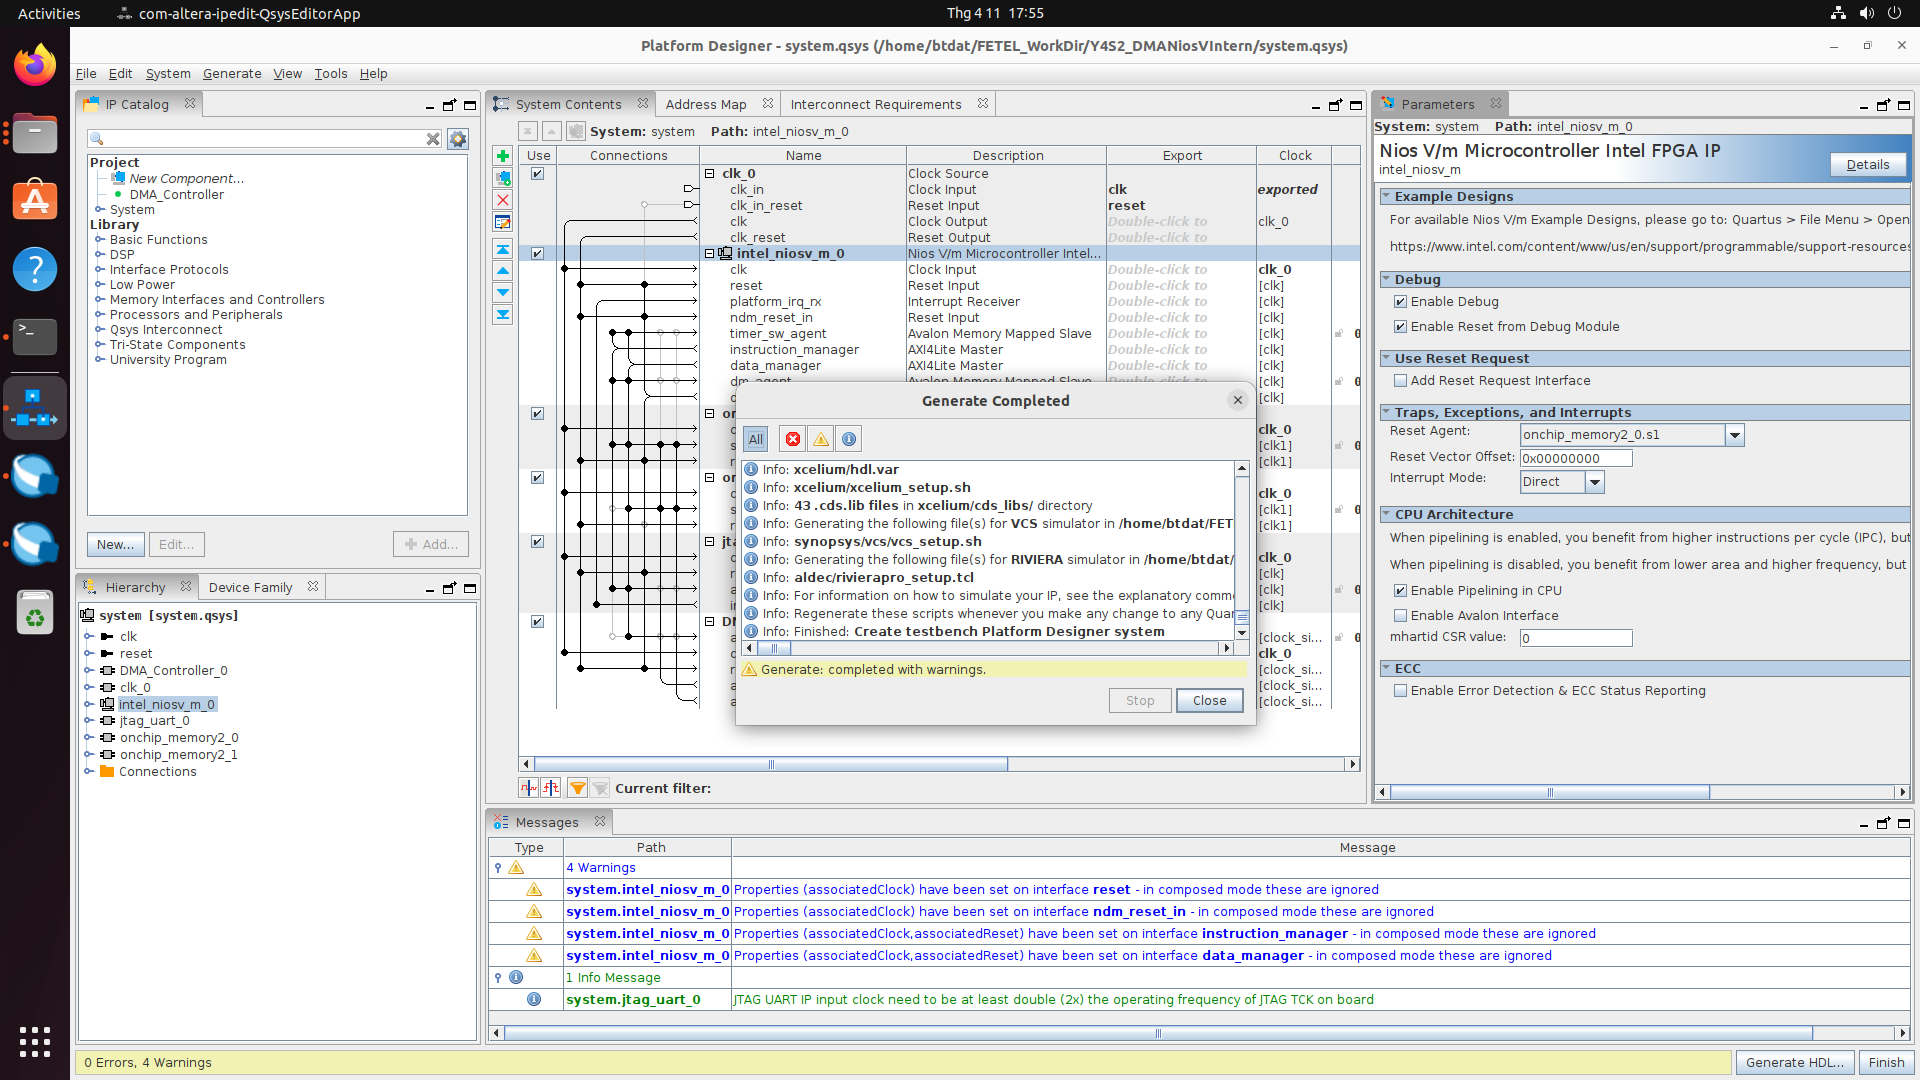
\includegraphics[width=\linewidth]{Images/04_01_UbuntuGenerateTestbenchSystem.png}
    \caption{Generate Testbench System trong Platform Designer trên Ubuntu 22.04.5 thành công.}
    \label{fig:04_01_UbuntuGenerateTestbenchSystem}
\end{figure}

Ngoài ra, để mô phỏng hoạt động của bộ xử lý \acrshort{niosv} chạy mã phần mềm, tệp chương trình thực thi (\texttt{.elf}) cần được biên dịch và chuyển đổi thành định dạng bộ nhớ (\texttt{.hex}) để nạp vào mô hình bộ nhớ trong quá trình mô phỏng.

\FloatBarrier

\section{Quy trình Thiết lập và Chạy Mô phỏng}

\begin{enumerate}
    \item \textbf{Tạo Testbench System:} Như đã đề cập, bước này cần thực hiện trên Linux dùng Platform Designer. Chọn File -> Generate Testbench System...
    \item \textbf{Chuẩn bị Thư mục Mô phỏng trên Windows:}
        \begin{itemize}
            \item Tạo một thư mục cho mô phỏng trên Windows (ví dụ: \texttt{D:\textbackslash ...\textbackslash DMANiosVIntern\_Sim}).
            \item Sao chép toàn bộ thư mục \texttt{testbench} được tạo bởi Platform Designer trên Linux vào thư mục mô phỏng trên Windows này. Cấu trúc thư mục sẽ tương tự như: \texttt{.../testbench/system\_tb/simulation/}.
        \end{itemize}
    \item \textbf{Biên dịch Phần mềm và Tạo file .hex:}
        \begin{itemize}
            \item Sử dụng Ashling RiscFree™ IDE (chạy từ Nios V Shell) để biên dịch dự án phần mềm C (thư mục \texttt{software/app}) như mô tả trong Chương \ref{Chapter3}. Thao tác này tạo ra tệp \texttt{app.elf}.
            \item Chạy lệnh sau trong Nios V Shell để chuyển đổi tệp \texttt{.elf} thành các tệp \texttt{.hex} cho bộ nhớ on-chip được sử dụng trong mô phỏng:
            \begin{lstlisting}[language=bash, caption={Command to generate .hex file from .elf}]
elf2hex --input=software/app/app.elf \
--output=system/testbench/system_tb/simulation/submodules/system_onchip_memory2_0.hex \
--base=0x20000 --end=0x3FFFF --width=32 --little-endian-mem --create-lanes=0

elf2hex --input=software/app/app.elf \
--output=system/testbench/system_tb/simulation/submodules/system_onchip_memory2_1.hex \
--base=0x40000 --end=0x5FFFF --width=32 --little-endian-mem --create-lanes=0
            \end{lstlisting}
            \textit{Lưu ý:} Các địa chỉ base (\texttt{--base}) và end (\texttt{--end}) phải khớp với địa chỉ của các khối \texttt{onchip\_memory2\_0} và \texttt{onchip\_memory2\_1} trong hệ thống Platform Designer. Các tệp \texttt{.hex} này sẽ được tự động đọc bởi testbench khi mô phỏng.
        \end{itemize}
    \item \textbf{(Nếu Di chuyển Testbench) Chỉnh sửa tệp TCL và C:}
        \begin{itemize}
            \item Mở tệp \texttt{<project\_dir>/system/testbench/system\_tb/simulation/msim\_setup.tcl}.
            \item Tìm và thay đổi đường dẫn thư viện QuestaSim từ định dạng Linux (\texttt{/}) sang định dạng Windows (\texttt{\textbackslash\textbackslash} hoặc \texttt{/}). Ví dụ: Thay đổi \texttt{D:/intelFPGA/23.1std/...} thành \texttt{D:/intelFPGA/23.1std/...} (thường thì dấu `/` vẫn hoạt động trên Windows trong TCL). Đảm bảo đường dẫn trỏ đến thư mục cài đặt QuestaSim chính xác trên máy Windows.
            \item Trong mã nguồn C (\texttt{hello\_world.c}), nếu có các định nghĩa \texttt{\#ifdef} dựa trên hệ điều hành (ví dụ: \texttt{\#ifdef linux}), chúng cần được điều chỉnh hoặc loại bỏ để đảm bảo mã hoạt động đúng trên Windows khi biên dịch cho mô phỏng.
        \end{itemize}
    \item \textbf{Chạy Mô phỏng bằng QuestaSim:}
        \begin{itemize}
            \item Mở QuestaSim.
            \item Trong cửa sổ Transcript, thay đổi thư mục làm việc đến thư mục \texttt{simulation} của testbench:
            \begin{lstlisting}[language=bash, caption={Setup QuestaSim environment}]
cd D:/FETEL_WorkDir/Y4S2_DMANiosVIntern_Sim/testbench/system_tb/simulation/
            \end{lstlisting}
            \item Thực thi tệp script cài đặt mô phỏng:
            \begin{lstlisting}[language=bash, caption={Run QuestaSim setup script}]
do msim_setup.tcl
            \end{lstlisting}
            Script này sẽ biên dịch các tệp Verilog/SystemVerilog cần thiết (bao gồm mã nguồn DMA, các IP hệ thống, và testbench) và nạp thiết kế.
            \item Nạp thiết kế cấp cao nhất và kích hoạt gỡ lỗi (nếu script chưa làm):
            \begin{lstlisting}[language=bash, caption={Load design and enable debug}]
ld_debug
            \end{lstlisting}
            \item Thêm các tín hiệu cần quan sát vào cửa sổ Wave:
            \begin{lstlisting}[language=bash, caption={Add signals to Wave window}]
# Example: Add all signals from the DMA controller
add wave -r sim:/system_tb/system_inst/dma_controller_0/*

# Or add specific signals and group them
add wave -divider "Control Slave"
add wave sim:/system_tb/system_inst/dma_controller_0/u_CONTROL_SLAVE/*
add wave -divider "Read Master"
add wave sim:/system_tb/system_inst/dma_controller_0/u_READ_MASTER/*
# ... (similarly for WRITE_MASTER, FIFO, and Avalon interfaces) ...
            \end{lstlisting}
            \item Chạy mô phỏng:
            \begin{lstlisting}[language=bash, caption={Run simulation}]
run -all
            \end{lstlisting}
        \end{itemize}
    \item \textbf{Phân tích Kết quả:} Quan sát các dạng sóng (waveforms) trong cửa sổ Wave để kiểm tra hoạt động của các tín hiệu điều khiển DMA, các giao dịch Avalon-MM, trạng thái FSM, và dữ liệu truyền qua FIFO. Kiểm tra output trong cửa sổ Transcript (từ các lệnh \texttt{printf} trong mã C thông qua mô hình JTAG UART) để xác minh kết quả truyền dữ liệu.
\end{enumerate}

Dạng sóng từ 3228702804 ps tới 3237620332 ps với argsimulationzero 

\begin{figure}
    \centering
    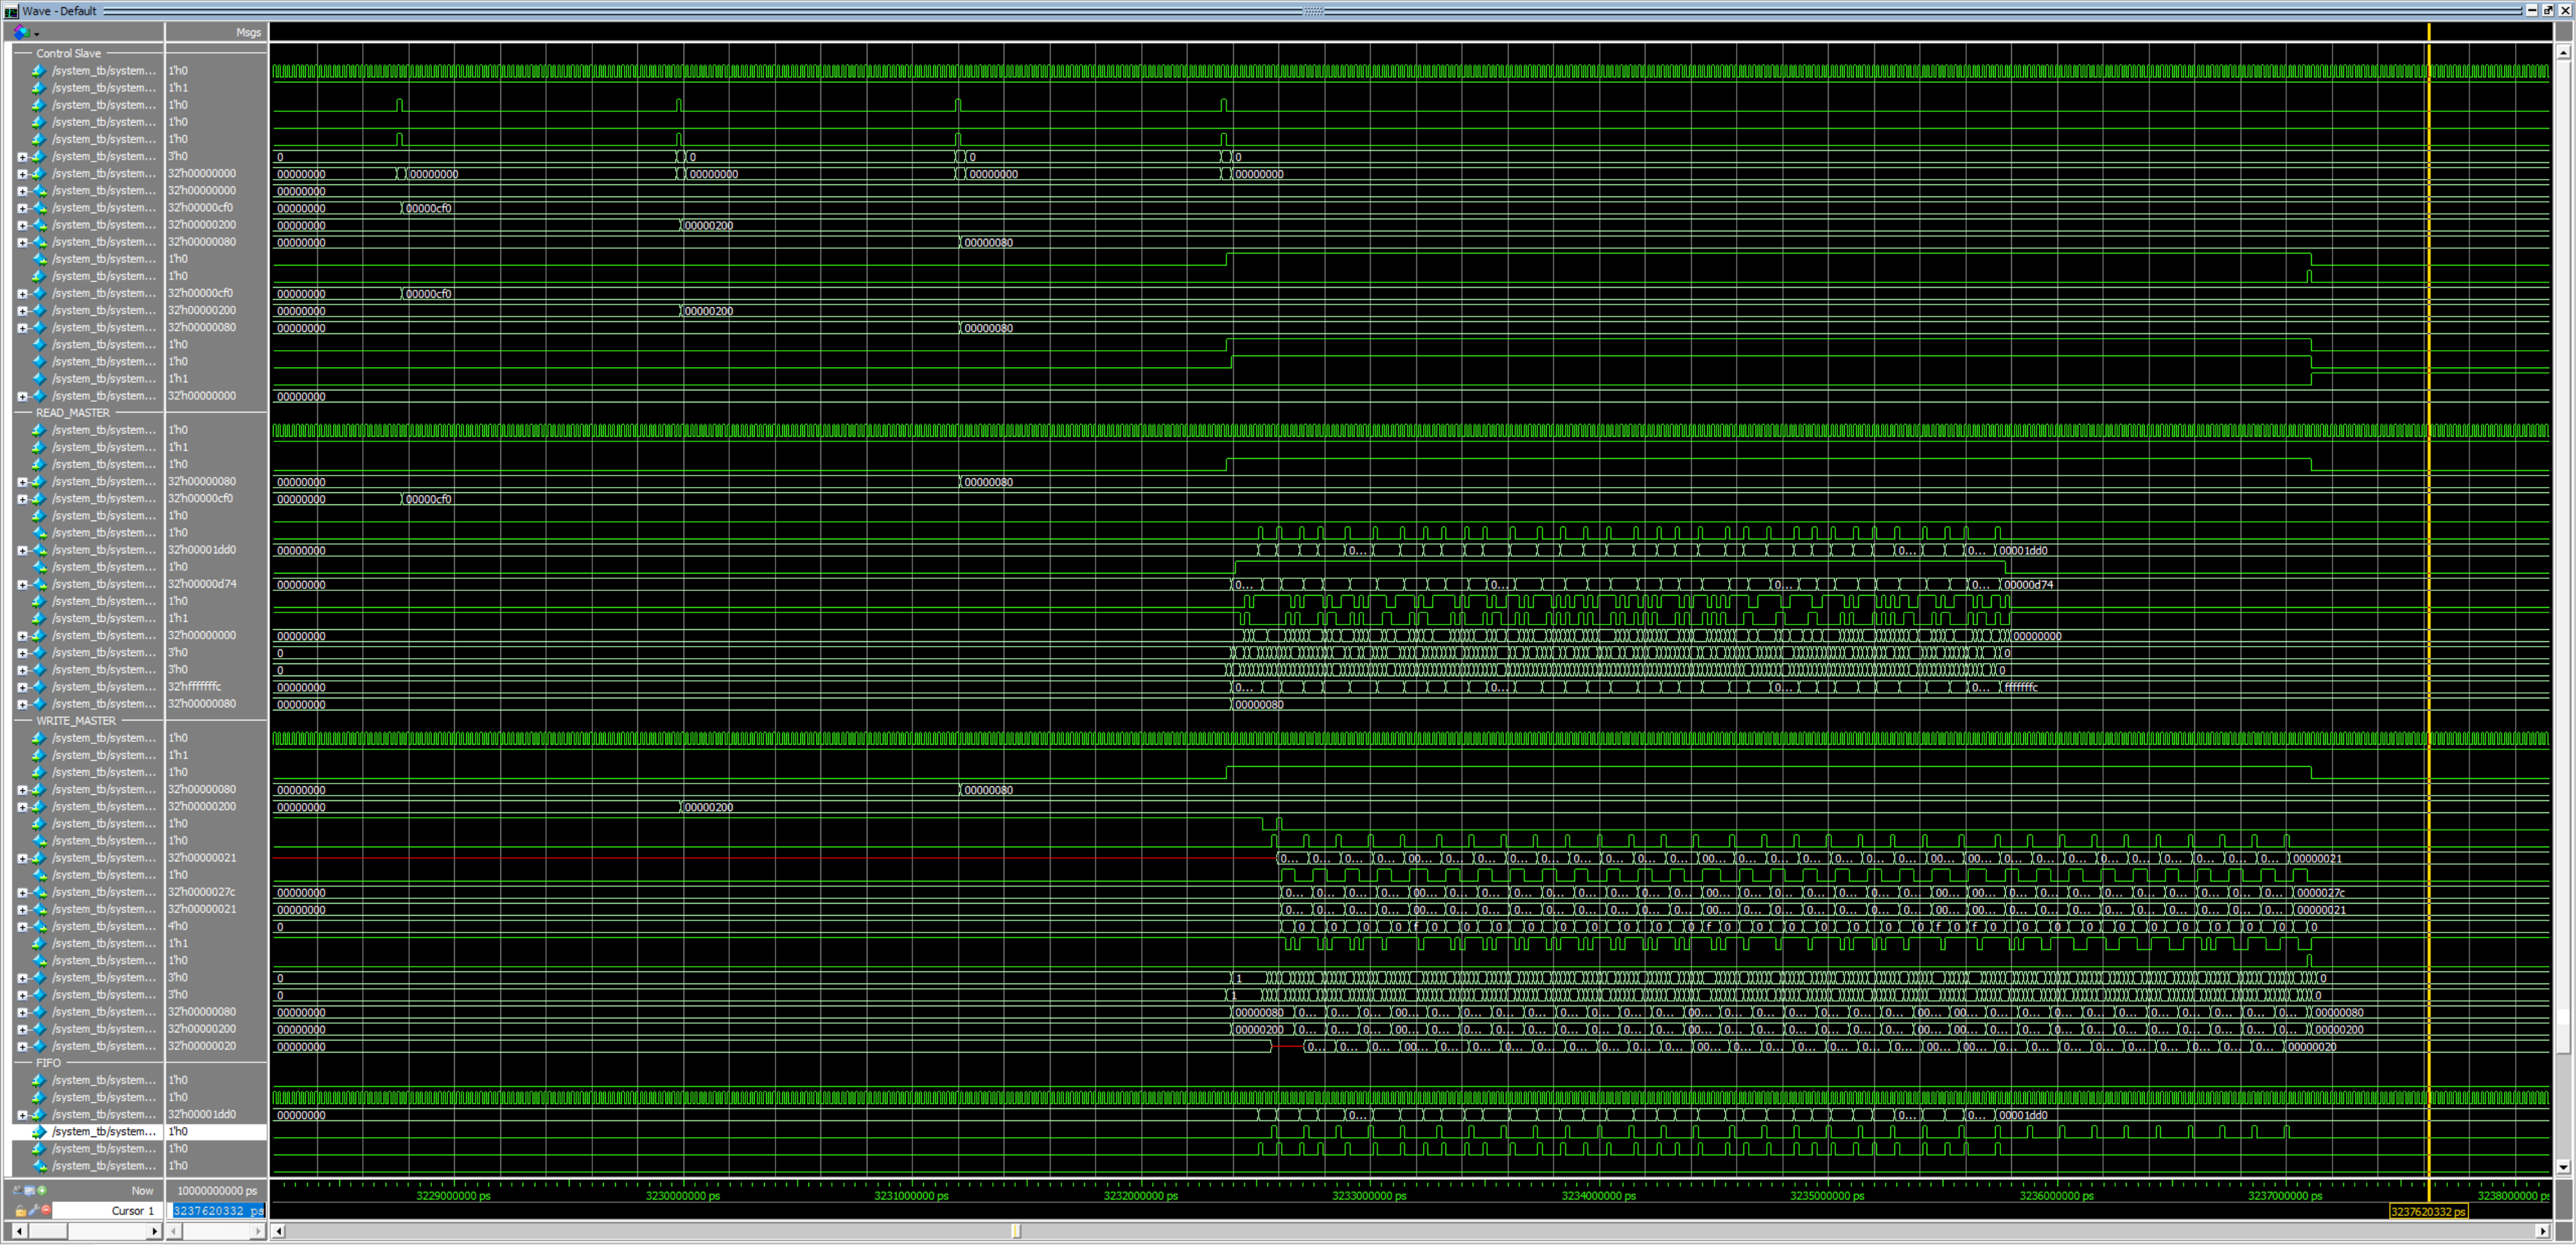
\includegraphics[width=\linewidth]{Images/04_03_QuestaSimWaveform_argsimulationzero.png}
    \caption{Dạng sóng mô phỏng cho các tín hiệu DMA và giao dịch Avalon-MM.}
    \label{fig:04_03_QuestaSimWaveform}
\end{figure}

\section{Gỡ lỗi Phần cứng với Signal Tap}

Bên cạnh mô phỏng, công cụ \textbf{Signal Tap Logic Analyzer} tích hợp trong Quartus Prime là một phương pháp hiệu quả để gỡ lỗi thiết kế trực tiếp trên phần cứng \acrshort{fpga}. Signal Tap cho phép chọn và quan sát các tín hiệu nội bộ trong thiết kế theo thời gian thực khi hệ thống đang chạy trên bo mạch.

Trong dự án này, Signal Tap có thể được sử dụng để:
\begin{itemize}
    \item Quan sát trạng thái của các FSM bên trong \texttt{READ\_MASTER} và \texttt{WRITE\_MASTER}.
    \item Theo dõi các giao dịch trên bus Avalon-MM (tín hiệu \texttt{read}, \texttt{write}, \texttt{address}, \texttt{readdata}, \texttt{writedata}, \texttt{waitrequest}, \texttt{readdatavalid}).
    \item Kiểm tra các tín hiệu điều khiển FIFO (\texttt{FF\_writerequest}, \texttt{FF\_readrequest}, \texttt{FF\_full}, \texttt{FF\_empty}).
    \item Xác minh tín hiệu \texttt{Start} và \texttt{WM\_done}.
\end{itemize}
Việc thiết lập Signal Tap bao gồm chọn các tín hiệu cần theo dõi (Nodes to Tap), thiết lập điều kiện kích hoạt (Trigger Conditions), và cấu hình bộ nhớ đệm (Buffer Depth). Sau khi biên dịch lại thiết kế với cấu hình Signal Tap, có thể sử dụng công cụ Signal Tap trong Quartus để nạp cấu hình và quan sát dạng sóng khi chạy ứng dụng phần mềm trên \acrshort{niosv}. Đây là một công cụ bổ trợ hữu ích cho mô phỏng, đặc biệt khi cần gỡ lỗi các vấn đề liên quan đến thời gian thực hoặc tương tác phần cứng phức tạp không dễ tái tạo trong mô phỏng.

% ----- END NEW Chapter 4 -----